% !TEX encoding = UTF-8 Unicode
\documentclass{article}

\usepackage{polski}
\usepackage[utf8]{inputenc}

\usepackage{graphicx}
\usepackage{subcaption}

\usepackage[a4paper, left=2.5cm, right=2.5cm, top=3.5cm, bottom=3.5cm, headsep=1.2cm]{geometry}

\linespread{1.3}

\begin{document}
	
	\begin{titlepage}
		\centering
		{\scshape\LARGE Politechnika Wrocławska \par}
		{\scshape\Large Katedra Informatyki Technicznej\par}
		\vspace{1cm}
		{\scshape\Large Bazy Danych 2\par}
		\vspace{1.5cm}
		{\huge\bfseries Domowa wypożyczalnia wideo\par}
		\vspace{2cm}
		{\Large\itshape Magdalena Biernat\par}
		{\Large\itshape Mateusz Bortkiewicz\par}
		\vfill\flushleft\large
		
		\normalsize	\centering	\vspace{3cm}
		Prowadzący\par
		dr inż. Tomasz Janiczek 
		
		\vfill
		{\large \today\par}
	\end{titlepage}
	\newpage
	\tableofcontents
	\newpage
		\section{Wprowadzenie}
	Niniejszy dokument powstał z myślą o projekcie na Bazy Danych 2. Jest to omówienie poszczególnych zagadnień jak i funkcjonalności stworzonej na potrzeby projektu aplikacji. 
	\section{Model konceptualny bazy danych}
	Poniżej przedstawiono model konceptualny naszej bazy. Zależało nam na tym, aby w bazie danych tabel było wystarczająco, tzn. była zaprezentowana każda relacja (jeden do jednego, jeden do wielu, wiele do wielu) oraz program implementował podstawowe funkcjonalności logowania i biblioteki. W tym celu posiadamy tabele skoncentrowane na samej bibliotece (Film, Specimen, Location etc), na użytkowniku (User, Inmate), oraz tabelę asocjacyjną wypożyczeń (Hire).
	\begin{figure}[!ht]	
		\centering
		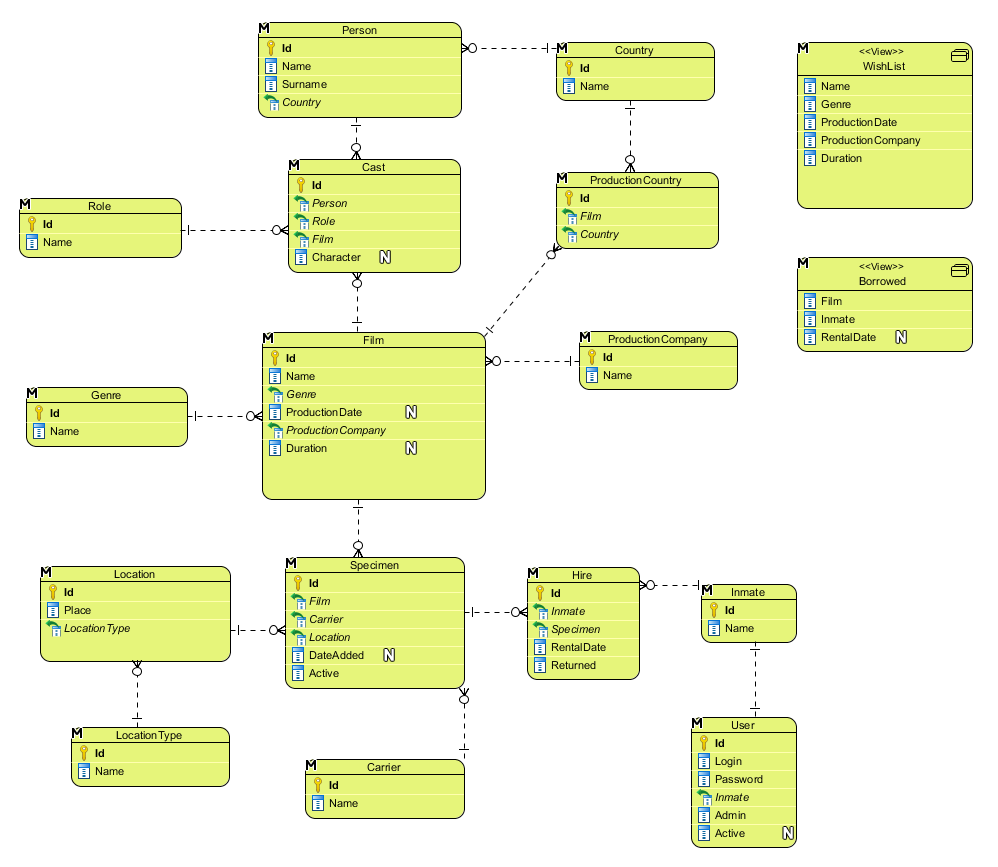
\includegraphics[height=13cm]{model_konceptualny.png}
		\caption{Model konceptualny}
		\label{fig:obrazek 0}
	\end{figure}
	\newpage
	\section{Opis "świata rzeczywistego"}
	Opis "świata rzeczywistego" - aplikacja "Domowa wypożyczalnia wideo"
	\subsection{Opis zasobów ludzkich}
	\begin{itemize}
		\item Głowa rodziny, tudzież osoba wyznaczona w domu administruje i zarządza aplikacją desktopową "Domowa wypożyczalnia wideo". Może ona usuwać i dodawać użytkowników, resetować hasła, zwracać/wypożyczać administracyjnie egzemplarze filmów, usuwać tytuły filmów, wycofywać z użycia egzemplarze filmów, a także wykonywać to co zwykły użytkownik
		\item Użytkownik, mieszkaniec domostwa może dodać lub edytować tytuły filmów oraz egzemplarze do tytułów obecnych już filmów. Może wypożyczać dostępny egzemplarz filmu
		\item Wypożyczenie posiada identyfikator domownika, identyfikator egzemplarza filmu a także datę wypożyczenia i informację czy film jest zwrócony.
		\item Użytkownik może edytować swoje konto, tj. zmieniać hasło.	
	\end{itemize}
	\subsection{Przepisy}
		Liczba wypożyczonych jednocześnie egzemplarzy przez danego użytkownika nie może być większa niż trzy. Nie istnieje termin zwrotu - wypożyczenie jest bezterminowe. Nieaktywny użytkownik nie może się zalogować na konto i wypożyczyć/zwrócić filmu.
	\subsection{Dane techniczne}
	\label{dane_techniczne}
		 Obsługa konta, bazy wideo i wypożyczeń powinna być dostępna przez aplikację desktopową połączoną z bazą danych.
		Wypożyczający loguje się do konta za pomocą loginu i hasła. Hasło nie jest przechowywane w bazie danych (jest to jedynie zasolone i haszowanie hasło).
	\newpage
	\section{Wymagania funkcjonalne i niefunkcjonalne}
	\subsection{Wymagania funkcjonalne}
	\begin{itemize}
	\item aplikacja ma mieć możliwość wyszukiwania\textbackslash dodawania\textbackslash edytowania\textbackslash usuwania filmów do bazy danych
	\begin{itemize}
		\item wyszukiwać i dodawać filmy może każdy użytkownik
		\item usuwać i edytować może tylko administrator systemu
	\end{itemize}
	\item aplikacja ma mieć możliwość edytowania danych użytkownika
	\item  dodawać nowego użytkownika może tylko administrator
	\item aplikacja ma mieć możliwość wyszukiwania\textbackslash dodawania\textbackslash edytowania\textbackslash usuwania tytułów filmów do bazy danych 
	\begin{itemize}
		\item wyszukiwać i dodawać tytuły może każdy użytkownik
		\item usuwać i edytować może tylko administrator systemu
	\end{itemize}
	\item obsadę może dodawać każdy użytkownik
	\item aplikacja pokazuje wypożyczone pozycje i listę życzeń (filmy, których egzemplarze nie są umieszczone w bazie danych)
	\end{itemize}
	\subsection{Wymagania niefunkcjonalne}	
	\begin{itemize}
		\item ilość domowników nie wpływa na szybkość działania systemu
		\item ilość filmów\textbackslash tytułów\textbackslash użytkowników etc. Jest ograniczona tylko pojemnością dysku na którym stoi baza danych
		\item przyjazny interfejs użytkownika
		\item liczba błędów w aplikacji przez pierwszy miesiąc od wydania aplikacji nie może przekroczyć 5		
	\end{itemize}
\newpage
	\section{Diagram przypadków użycia}
	W diagramie przypadków użycia, podzieliliśmy funkcjonalności programu na klasy (Użytkownicy, Filmy, Tytuły, etc.) i wystosowaliśmy dla każdego obszaru po kilka funkcjonalności, po między którymi zachodzą relacje Include i Extend. Diagram w pełnej rozdzielczości można znaleźć w programie załączonym do niniejszego sprawozdania.
	\begin{figure}[!ht]	
		\centering
		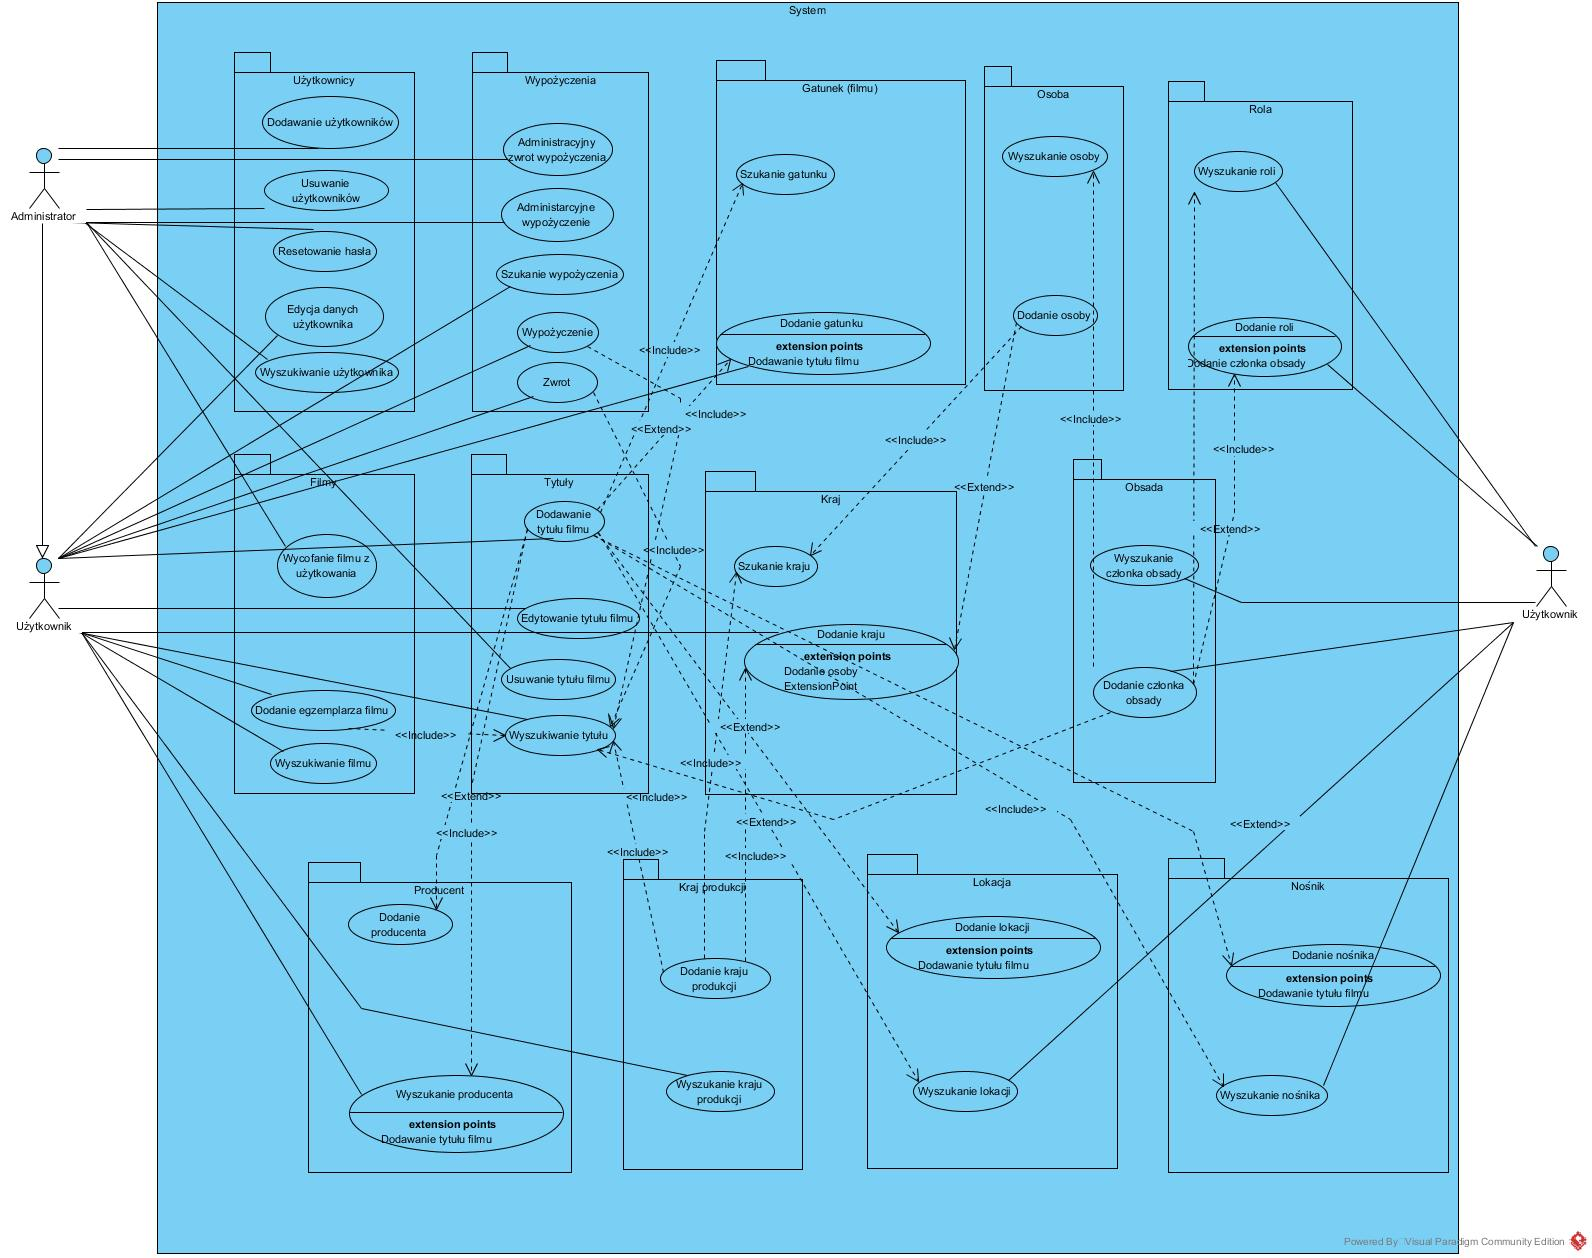
\includegraphics[height=13cm]{PU.jpg}
		\caption{Diagram przypadków użycia}
		\label{fig:obrazek 1}
	\end{figure}
\newpage
	\section{Diagram związków encji}
	Podczas tworzenia diagramu związków encji, kierowaliśmy się przedstawionym wcześniej modelem konceptualnym. Diagram związków encji, w stosunku do modelu konceptualnego został uzupełniony o typy danych dla poszczególnych pól w tabelach.
		\begin{figure}[!ht]	
		\centering
		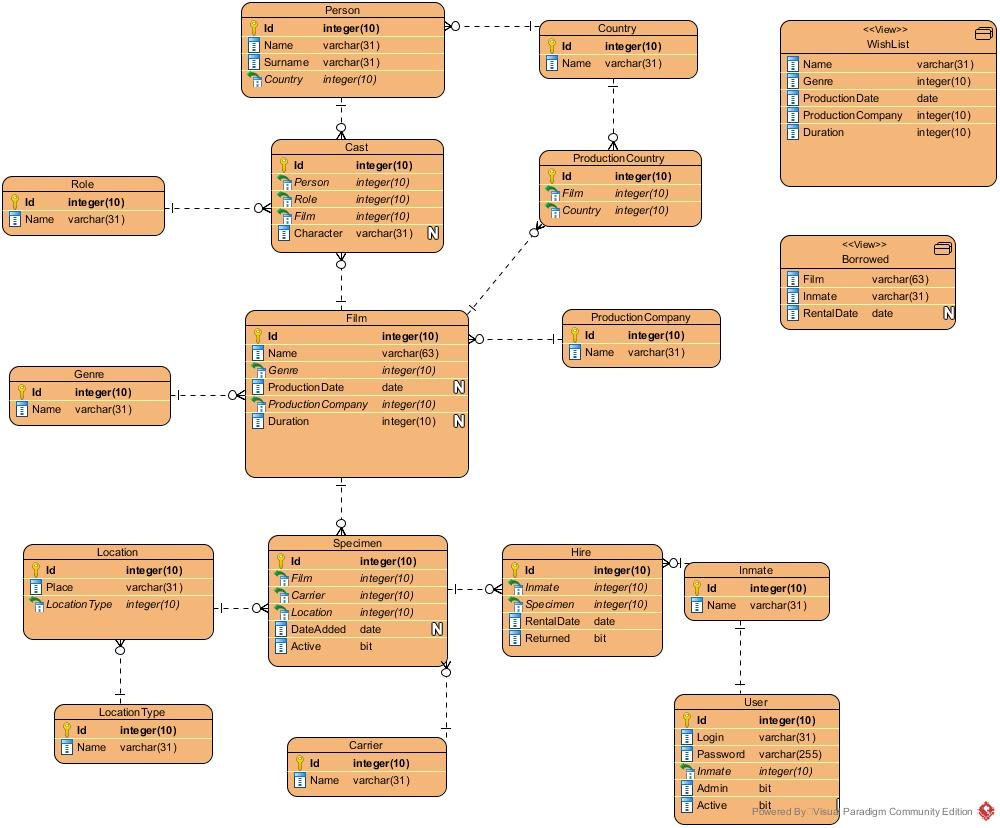
\includegraphics[height=14cm]{diagram_zwiazkow_encji.jpg}
		\caption{Diagram związków encji}
		\label{fig:obrazek 2}
	\end{figure}
\newpage
\section{Analiza ilości encji}
\subsection{Analiza liczby instancji dla każdej encji}
\begin{itemize}
\item Film – ok. 50 rekordów (przykładowo)
\item Specimen – ok. 50 rekordów (podobnie jak Film)
\item Carrier (nośnik) – 5-10 rekordów ( Nie więcej jak Specimen)
\item LocationType (typ lokacji) – 5-10 rekordów (nie więcej jak Location)
\item Location (lokacja) – ok. 50 rekordów (nie więcej jak Specimen)
\item Hire (wypożyczenie) – 10 na sam początek , nie więcej jak 3 * liczba użytkowników
\item Inmate (domownik) – ok. 10 rekordów
\item User (użytkownik) – ok.10 rekordów (tak samo jak Inmate)
\item ProductionCompany (Wytwórnia filmów) – ok. 10-15 rekordów
\item Person (osoba)– minimalnie ilość rekordów 1 per Film (przykładowo)
\item Cast (obsada) – maksymalnie Person * Role * Film
\item Role (rola w filmie) – ok. 10 rekordów (przykładowo)
\item Contry (kraj) – maksymalnie ok. 240, minimalnie 1
\item ProductionCountry (Kraj produkcji) – maksymalnie Contry * Film
\item Genre (gatunek) – ok. 15 rekordów (przykładowo)
\end{itemize}

\subsection{Analiza użycia dla każdej encji}
\begin{itemize}
\item Film – wyszukiwanie najczęściej, potem dodawanie i edycja, prawie wcale usuwanie
\item Specimen - wyszukiwanie najczęściej, potem dodawanie i edycja, prawie wcale usuwanie
\item Carrier – wyszukiwanie najczęściej, rzadziej dodawanie (najwięcej rekordów na początku istnienia bazy), prawie wcale edycja, brak usuwania
\item LocationType – wyszukiwanie najczęściej, potem dodawanie, brak usuwania i edycji
\item Location – wyszukiwanie najczęściej, podobnie dodawanie, najmniej edycja, brak usuwania
\item Hire – wyszukiwanie i dodawanie najczęściej, podobnie usuwanie, brak edycji
\item Inmate – wyszukiwanie najczęściej, rzadziej dodawanie, brak edycji i usuwania
\item User – wyszukiwanie najczęściej, rzadziej dodawanie i edycja, brak usuwania
\item ProductionCompany – wyszukiwanie najczęściej, potem dodawanie, brak edycji i usuwania
\item Person – wyszukiwanie najczęściej, potem dodawanie, brak edycji i usuwania
\item Cast – najczęściej wyszukiwanie, potem dodawanie, brak edycji, rzadko usuwanie
\item Role – najczęściej wyszukiwanie, rzadko dodawanie (najwięcej rekordów na początku istnienia bazy), brak edycji i usuwania
\item Country – najczęściej wyszukiwanie, rzadko dodawanie, (najwięcej rekordów na początku istnienia bazy) brak edycji i usuwania
\item ProductionCountry  - najczęściej wyszukiwanie, potem dodawanie, rzadko edycja, brak usuwania
\item Genre – najczęściej wyszukiwanie, rzadko dodawanie (najwięcej rekordów na początku istnienia bazy), brak usuwania i edycji

\end{itemize}
\section{Implementacja bazy danych}
\begin{figure}[!ht]
\centering
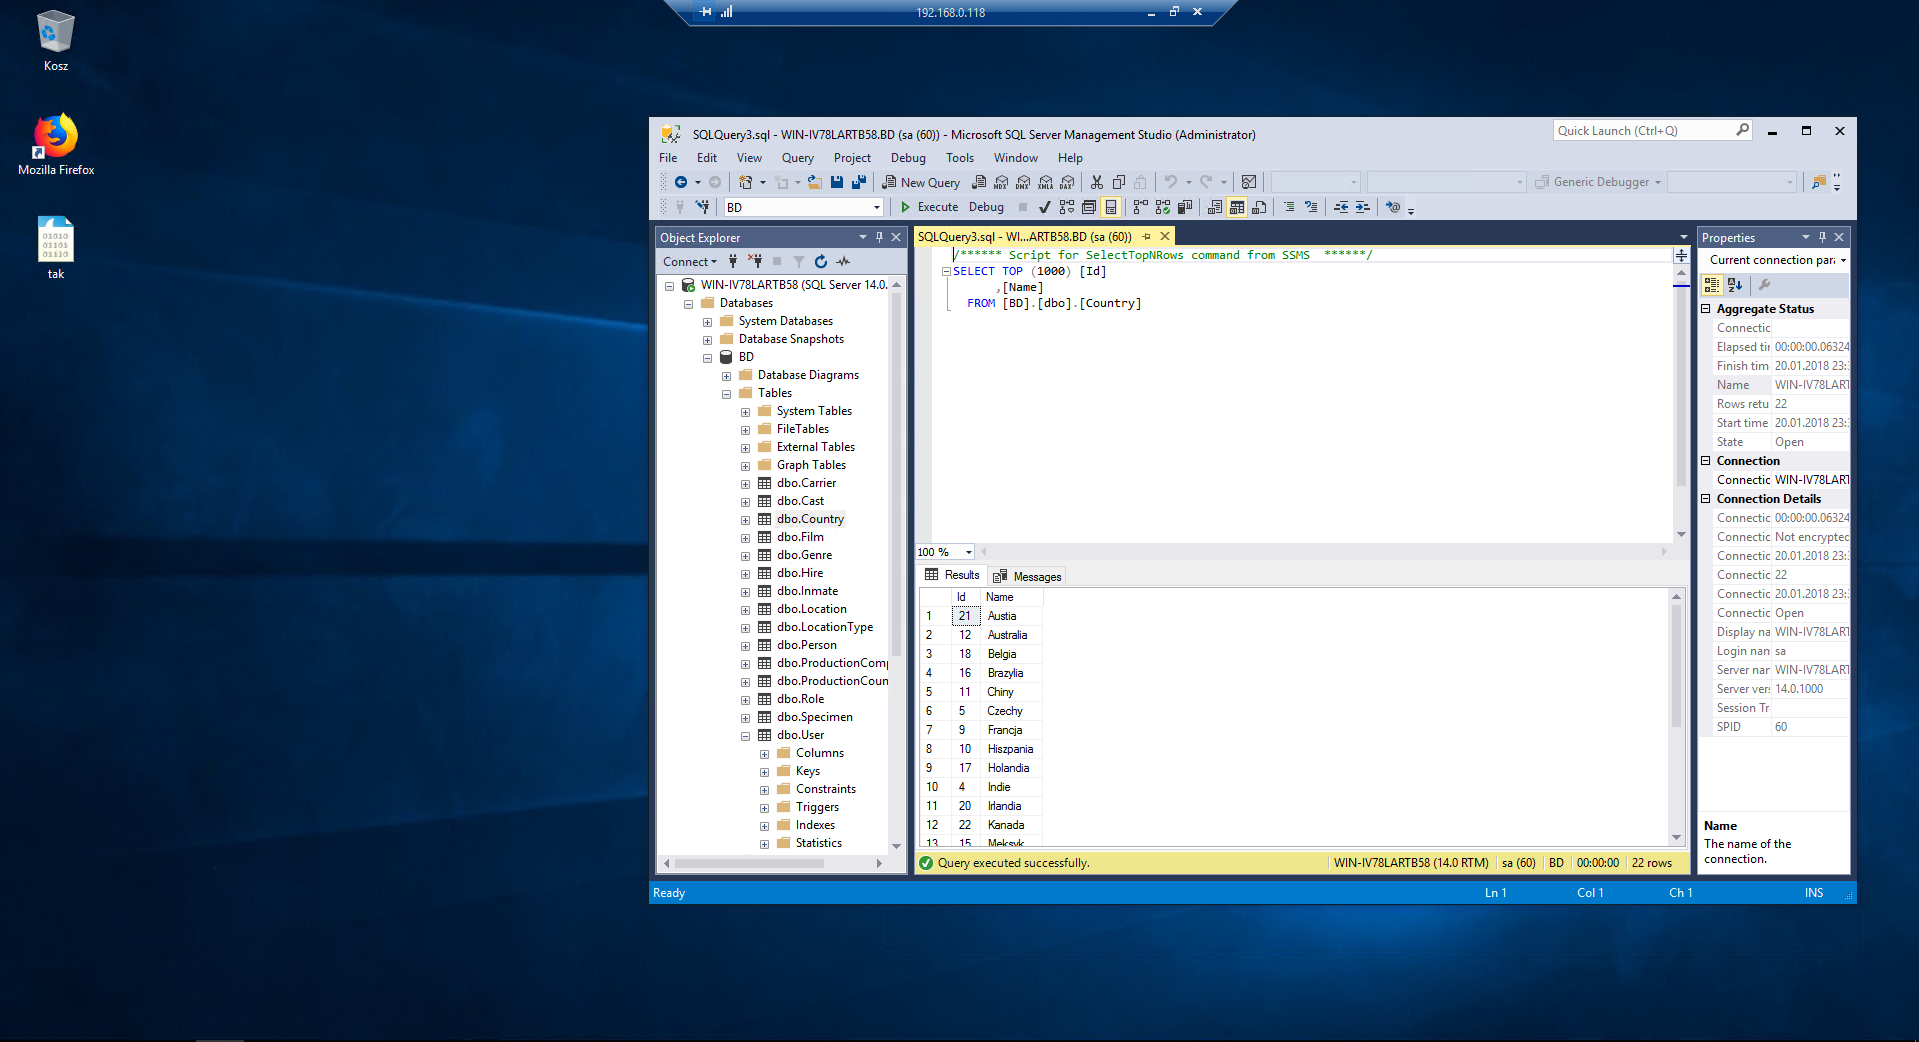
\includegraphics[width=15cm]{serwer.PNG}
\caption{Serwer na maszynie wirtualnej}
\end{figure}
\subsection{Serwer bazodanowy}
W związku z chęcią realizacji aplikacji na platformie .NET, zdecydowaliśmy się na wybór instancji bazodanowej dostarczonej przez firmę Microsoft, a mianowicie MS SQL Server 2017 w wersji Developer. Do jej zarządzania będziemy używać dostarczonego w pakiecie narzędzia - Management Studio, bądź też przeglądarki wbudowanej w środowisko programistyczne - Visual Studio 2015. Instancja serwera bazodanowego będzie umieszczona na maszynie wirtualnej (postawionej w środowisku VM VirtualBox) w systemie operacyjnym Microsoft Windows Server 2016 Standard. Aby umożliwić prostszą konfigurację, dostęp do serwera będzie odbywał się z poziomu aplikacji Pulpitu Zdalnego. W celu użycia bazy danych w aplikacji na innym komputerze, odblokowano port 1433 na zaporze sieciowej serwera, odpowiadający za nasłuchiwanie połączeń przychodzących.  
\subsection{Tworzenie tabel i wprowadzanie danych}
Tabele stworzono wg diagramów związków encji. Zawierają one przykładowe dane, niekoniecznie zgodne z rzeczywistością. Dla ułatwienia, tabeli zawierającej wypożyczenia, a także pola HashedPassword w tabeli Users nie wypełniono - będą one użyte, jak również wypełnione, podczas testów aplikacji w etapie III. Skrypt tabeli zamieszczony jest w załączniku.
\section{Polityka bezpieczeństwa}
\subsection{Zabezpieczenie serwera}
W celu zwiększenia bezpieczeństwa, dostęp do instancji bazodanowej będzie chroniony, tzn. aby się z nią połączyć potrzebne będzie hasło. Instancja posiada domyślny profil administratora (sa) oraz hasło dostarczone przez twórcę aplikacji (na potrzeby projektu, hasłem jest BazyDanych@2). Nie jest wymagane tworzone dodatkowych kont do instancji.
\subsection{Dostęp do kont użytkowników}
Jak to zostało wspomniane w danych technicznych w punkcie \ref{dane_techniczne}, hasła użytkowników planujemy szyfrować. Myślimy o wykorzystaniu szyfrowania symetrycznego. Jako iż będziemy korzystać z platformy .NET, do naszych celów wykorzystamy gotową klasę CryptoStream biblioteki System.Security.Cryptography, która pozwoli nam przekształcać hasło, na niezrozumiały ciąg znaków. Wykorzystuje ona szyfrowanie \textit{AES} (ang. Advanced Encryption Standard). 
\subsection{Sniffing}
Przeprowadzono test bezpieczeństwa na serwerze z użyciem programu \textit{Wireshark}. Celem było przechwycenie danych przychodzących lub wychodzących z instancji bazodanowej. Stwierdzono iż MSSQL Server przesyła dane za pomocą protokołu \textit{TDS} (Tabular Data Stream) w formie odkrytej, tzn. za pomocą Wireshark'a jesteśmy w stanie przechwycić dane przychodzące (wysłane zdalnie zapytania), jak i wychodzące (wysyłane dane w zapytaniu). Test również wykazał iż nie jesteśmy w stanie określić hasła do serwera bazodanowego, tzn. cześć pakietów jest zaszyfrowana. Warto zaznaczyć również iż zabezpieczenie wskazane w poprzednim podpunkcie zabezpiecza hasło podczas przesyłania, tzn. jest ono przesyłane tylko w formie znanej aplikacji. 
\begin{figure}[!ht]
\centering
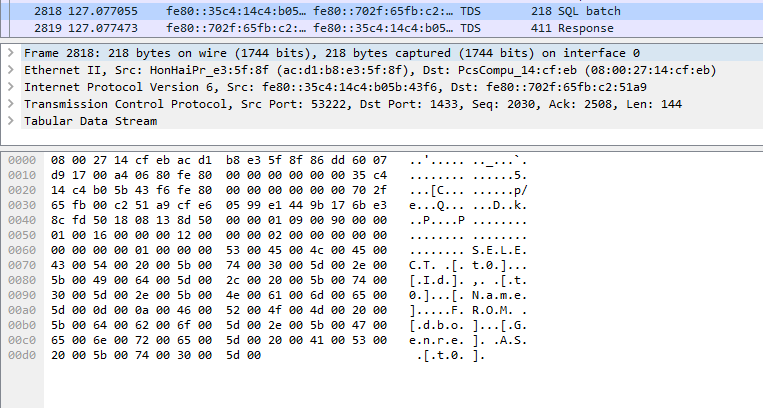
\includegraphics[width=15cm]{odebrane.PNG}
\caption{Odebrany pakiet (zapytanie)}
\end{figure}
\newpage
\begin{figure}[!h]
\centering
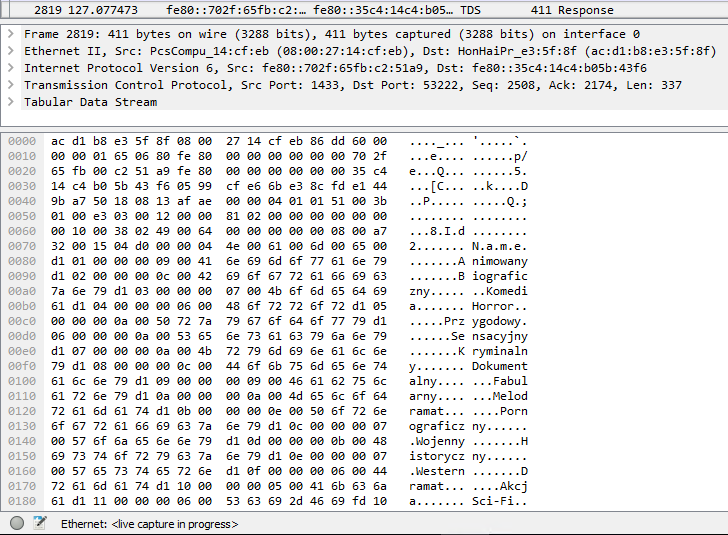
\includegraphics[width=15cm]{wyslane.PNG}
\caption{Wysłany pakiet (dane w odpowiedzi na zapytanie)}
\end{figure}

Podsumowując podpunkt, zabezpieczenia zastosowane w programie są wystarczające, tzn. nawet w przypadku sniffingu nie jesteśmy w stanie odczytać wrażliwych danych (haseł) ze względu na zastosowane zabezpieczenia przy budowie projektu (haszowanie hasła) i przez protokoły serwera bazodanowego (szyfrowanie wrażliwych pakietów).

Należy też zauważyć, iż dostęp do bazy danych z poza sieci domowej (lokalnej) nie będzie możliwy (aplikacja pracuje tylko w sieci lokalnej), a co za tym idzie, ryzyko włamania do bazy danych bliskie zeru.
\section{Aplikacja desktopowa}
\subsection{Środowisko i wykonanie}
Program został napisany w środowisku Visual Studio 2015 na platformie .NET z użyciem języka C\# i interfejsu Windows Forms. Do komunikacji z bazą danych używamy technologii LINQ to SQL, mapującej bazy danych relacyjne na obiektowe. Znaczy to mniej więcej, że mając bazę danych opartą na relacjach, jesteśmy w stanie odwoływać się do poszczególnych rekordów tabel jak do obiektów poszczególnych klas. Poprzez odwołanie do klasy \textit{Database} jesteśmy w stanie wydobyć za pomocą chociażby wyrażenia lambda interesujący nas zestaw rekordów. Dla przykładu:
\begin{verbatim}
Database.Current.Genres.Where(g => g.Name.ToLower() == name.ToLower()).ToList();
\end{verbatim}
wyrażenie lambda zwraca takie obiekty klasy Genres, których nazwa (\textit{Name}) reprezentowana przez małe litery jest taka sama jak zadany parametr \textit{name}.
\subsection{Struktura projektu}
Projekt jest podzielony wg wzorca \textit{MVC} (Model-View-Controler). Są to 3 warstwy, które są odpowiedzialne za strukturę aplikacji. Każda z warstw posiada swój osobny folder, w którym są wydzielone odpowiednie klasy. W przypadku klas z Modelu i Kontrolera, wykorzystujemy klasy typu partial, jest są to pojedyncze klasy, ale rozbite na kilka plików. 
\begin{itemize}
\item Model odpowiada za warstwę danych, ich struktury. Są to m.in. klasy wygenerowane przez plik .dbml oraz stworzony enum \textit{Result}.
\item Controller jest odpowiedzialny za przetwarzanie danych. Warstwa ta pobiera i przetwarza dane z bazy danych i wysyła odpowiednie odpowiedzi do warstwy Widoku.
\item View (Widok) odpowiada za graficzną prezentację, a więc w tej warstwie znajdować się będą wszystkie definicje okien i akcje związane z posiadanymi kontrolkami.
\end{itemize}
\newpage
\begin{figure}[!ht]
\centering
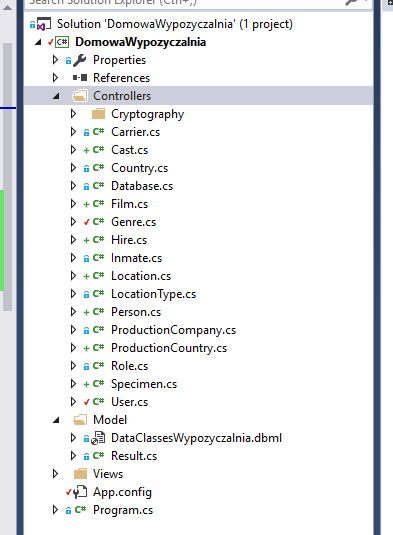
\includegraphics[width=8cm]{mvc.PNG}
\caption{Struktura projektu wg wzorca MVC}
\end{figure}
\subsection{Połączenie z bazą danych}
Aby się połączyć z bazą danych, w pliku \textit{app.config} został umieszczony \textit{ConnectionString}, który posiada podstawowe dane nt. łączenia się z bazą danych.
\begin{verbatim}
    <connectionStrings>
        <add name="DomowaWypozyczalnia.Properties.Settings.BDConnectionString"
            connectionString="Data Source=WIN-IV78LARTB58;Initial Catalog=BD;
                                  User ID=sa;Password=BazyDanych@2;"
            providerName="System.Data.SqlClient" />
    </connectionStrings>
\end{verbatim}
Gdzie sekcja \textit{name} to jest nazwa tego ConnectionStringa, sekcja \textit{connectionString} posiada informacje, kolejno; nazwę instancji bazodanowej, nazwę bazy danych, a także login i hasło użytkownika. W sekcji \textit{providerName} deklarujemy natomiast, że instancja bazodanowa jest dostarczona przez Microsoft i korzystamy z przestrzeni nazw \textit{System.Data.SqlClient}.
\subsection{Logowanie do aplikacji}
Logowanie do aplikacji odbywa się za pomocą loginu i hasła. Pole hasło ma ustawioną właściwość \textit{PasswordChar} na \textit{true}, a co za tym idzie - hasło jest niewidoczne podczas jego wpisywania.
\begin{figure}[!ht]
\centering
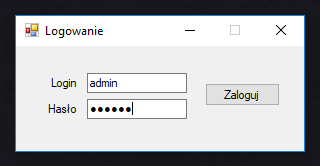
\includegraphics[width=8cm]{logowanie.PNG}
\caption{Okno logowania}
\end{figure}

Tak zatwierdzone login i hasło są sprawdzane przez program pod kątem poprawności. Jeśli nie istnieje użytkownik o zadanym loginie, wyświetlany jest stosowny komunikat. W przypadku gdy użytkownik istnieje, ale hasło nie jest poprawne, wyświetlany jest komunikat o innej treści. Użytkownik oznaczony w bazie danych jako nieaktywny, a pragnący się zalogować do systemu, otrzyma komunikat o niepoprawnym loginie - próba zalogowania się takiej persony, traktowana jest jak wpisanie nieprawidłowego loginu.

\begin{figure}[!ht]
\centering
  \begin{subfigure}[b]{0.3\textwidth}
  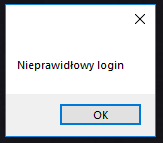
\includegraphics[width=\textwidth]{login.PNG}
  \caption{Niepoprawnie wpisany login}
  \end{subfigure}
  \begin{subfigure}[b]{0.3\textwidth}
  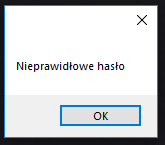
\includegraphics[width=\textwidth]{haslo.PNG}
  \caption{Niepoprawnie wpisane hasło}
  \end{subfigure}
  \caption{Komunikaty o braku poprawności}
\end{figure}
\newpage
\subsection{Okno główne}
\subsubsection{Panel użytkownika}
\begin{figure}[!ht]
\centering
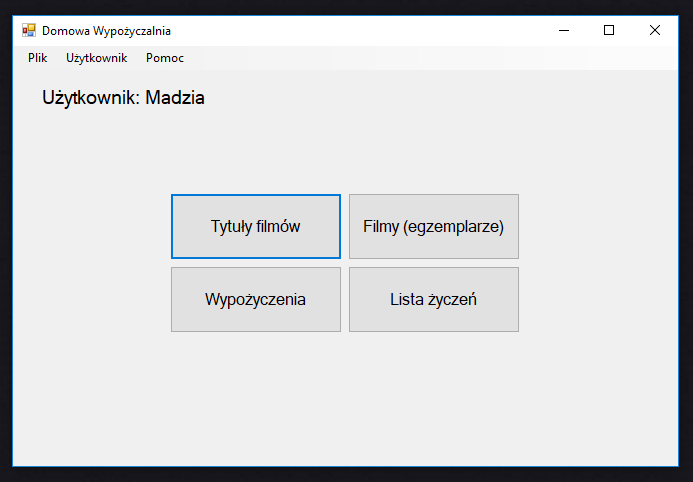
\includegraphics[width=12cm]{userwindow.PNG}
\caption{Interfejs użytkownika}
\end{figure}
Jak widać, użytkownik ma wgląd w tytuły filmów, w poszczególne egzemplarze filmów, w aktualne (swoje) wypożyczenia i w listę życzeń, czyli te tytuły filmów, które nie posiadają egzemplarzy. W menu, na pasku, posiadamy pozycje: Plik (a tam opcję Zamknij), Użytkownik (zmień dane) oraz Pomoc (o programie).
\newpage
\subsubsection{Panel administratora}
\begin{figure}[!ht]
\centering
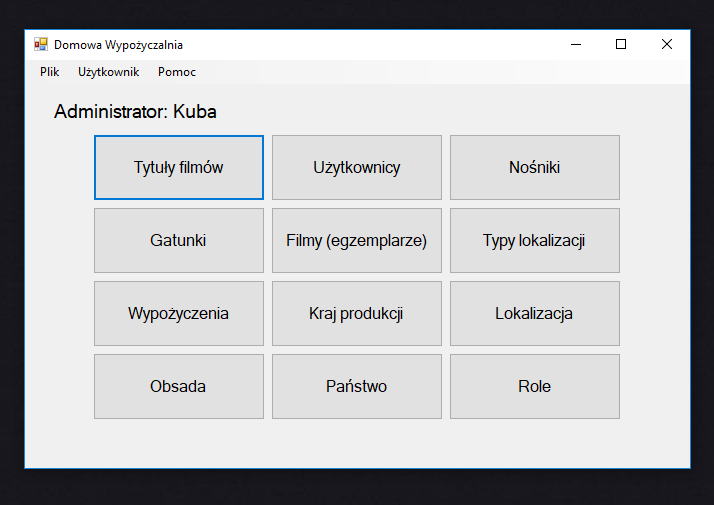
\includegraphics[width=12cm]{adminwindow.PNG}
\caption{Interfejs administratora}
\end{figure}
Administrator posiada podobnie jak użytkownik, wgląd w Tytuły filmów, w same Filmy, ale też w Wypożyczenia wszystkich użytkowników oraz samych użytkowników. Może przeglądać, dodawać, usuwać i edytować Nośniki, Gatunki, Lokalizacje, Państwa, Kraje produkcji, Obsady itd. Ponadto na pasku menu posiada to samo co normalny użytkownik.
\subsection{Funkcjonalności}
Jeśli chodzi o poszczególne opcje dostępne w programie:
\begin{itemize}
\item Tytuły filmów - w oknie dostępna jest możliwość wyświetlenia, a także dodania nowych tytułów filmowych, a także aktorów. Tylko administrator posiada prawo edycji tytułu filmowego i aktora.
\item Użytkownicy - opcja dostępna u administratora. Może resetować hasło dowolnych użytkowników, oznaczać ich jako nieaktywnych.
\item Nośniki - opcja dostępna u administratora. Umożliwia wyświetlenie, dodanie, edycję i usunięcie dowolnego nośnika.
\item Gatunki (filmowe) - opcja dostępna u administratora. Umożliwia wyświetlenie, dodanie, edycję i usunięcie dowolnego gatunku.
\item Filmy (egzemplarze) - w oknie jest możliwość dodania nowych egzemplarzy istniejących już tytułów. Administrator może je edytować i oznaczać jako nieaktywne.
\item Typy lokalizacji - opcja dostępna u administratora. Umożliwia wyświetlenie, dodanie, edycję i usunięcie dowolnego typu lokalizacji.
\item Wypożyczenia - umożliwia przeglądanie aktywnych wypożyczeń i dokonanie zwrotu wypożyczonej pozycji. Administrator może przeglądać wypożyczenia wszystkich użytkowników i dokonywać administracyjnego zwrotu.
\item Kraj produkcji - opcja dostępna u administratora. Umożliwia przypisanie kraju do dowolnego filmu jako kraju produkcji. Wyświetla wszystkie powiązania.
\item Lokalizacja - opcja dostępna u administratora. Umożliwia wyświetlenie, dodanie, edycję i usunięcie lokalizacji. 
\item Obsada - opcja dostępna u administratora. Umożliwia wyświetlenie, dodanie, edycję i usunięcie aktorów przypisanych do danych filmów.
\item Państwo - opcja dostępna u administratora. Umożliwia wyświetlenie, dodanie, edycję i usunięcie państwa z bazy danych.
\item Role - opcja dostępna u administratora. Umożliwia wyświetlenie, dodanie, edycję i usunięcie możliwych ról w filmach.
\end{itemize}
\subsection{Tytuły filmów}
Okno posiada dwa komponenty typu \textit{dataGridView}, umieszczonych w różnych groupBoxach. W pierwszym, znajdziemy wszystkie filmy z naszej bazy danych w kolejności chronologicznej jeśli chodzi o ich dodanie. W zależności od zaznaczonego wiersza, w polach obok będą się zmieniać dane. W drugim komponencie ukażą się nam aktorzy grający w danym filmie, oczywiście jeśli tacy występują. Podobnie tutaj po prawej stronie mamy pola, które będą nam pokazywać parametry danej postaci z filmu. Dodatkowo, mamy możliwość dodania nowego filmu, a także nowego aktora do filmu, aktualnie widnieje w zaznaczeniu. Administrator może wyedytować zaznaczoną postać i dany film oraz je usunąć. W przypadku usunięcia filmu szukamy, czy dany film nie posiada powiązań z innym rekordem. Jeśli nie ma ich, możemy śmiało usuwać rekord. 
\begin{figure}[!ht]
\centering
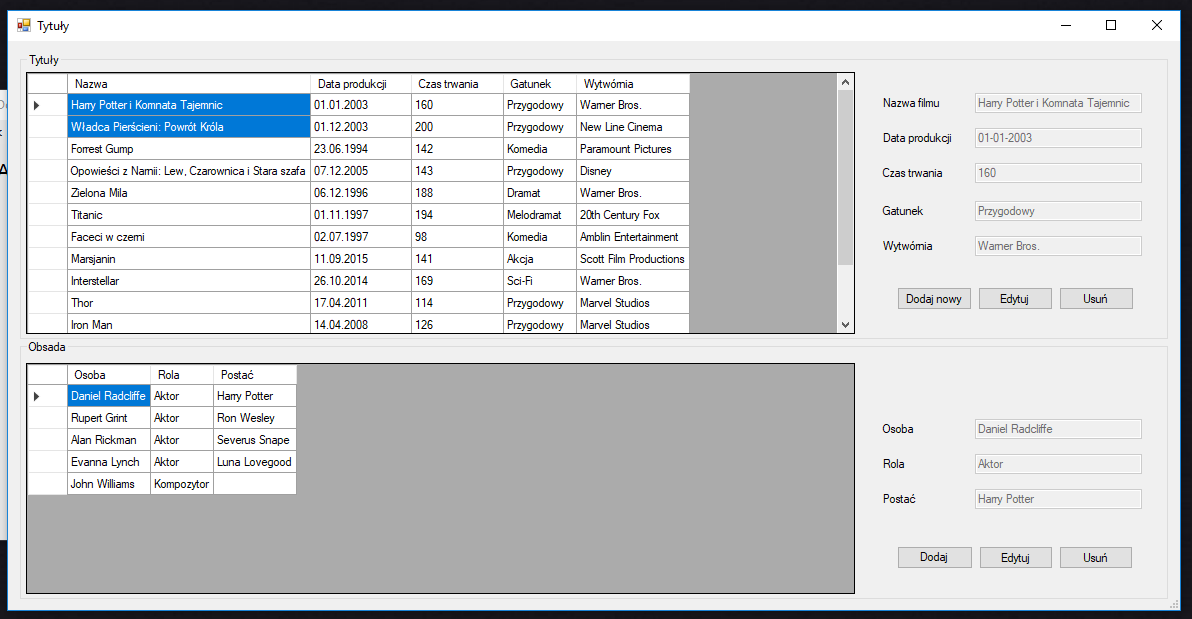
\includegraphics[width=12.5cm]{tytuly.PNG}
\caption{Stworzone okno z tytułami filmów}
\end{figure}

Podobnym oknem będzie lista życzeń. W tym przypadku nie będziemy mieć opcji edycji i usuwania. W stosunku do okna tytułów filmów różni się tym, że w zapytaniu są zwracane te rekordy, które posiadają powiązanie z tabelą \textit{Specimen}.
\subsection{Użytkownicy}
Okno jest tylko do dyspozycji administratora. Można obejrzeć w nim wszystkich użytkowników, dodać nowych, edytować i oznaczać jako nieaktywnych bądź aktywnych. Okno posiada również opcję filtrowania. Jeśli chcemy zobaczyć tylko użytkowników aktywnych, zaznaczamy kontrolkę checkBox i odświeża nam się widok. W przypadku oznaczania jako nieaktywny - okno posiada blokadę, ażeby jednocześnie istniał co najmniej jeden aktywny administrator.
\begin{figure}[!ht]
\centering
  \begin{subfigure}[b]{0.45\textwidth}
  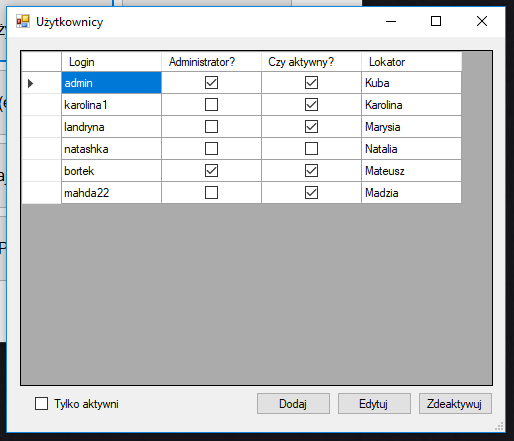
\includegraphics[width=\textwidth]{users.PNG}
  \caption{Wszyscy użytkownicy}
  \end{subfigure}
  \begin{subfigure}[b]{0.45\textwidth}
  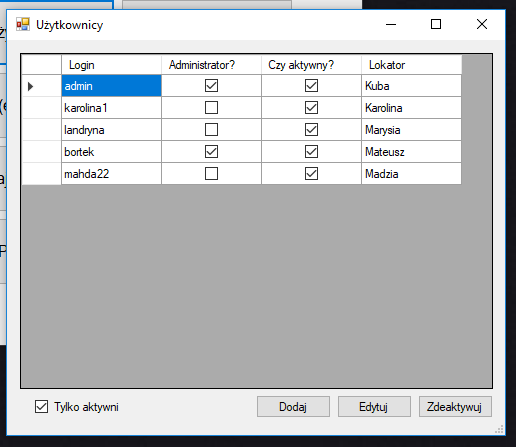
\includegraphics[width=\textwidth]{active.PNG}
  \caption{Aktywni użytkownicy}
  \end{subfigure}
  \caption{Okno Użytkownicy}
\end{figure}
\subsection{SingleProperty}
Są to okna, w których edytujemy, dodajemy tylko jedną właściwość. Będą się tyczyć tabel tj. Carrier (Nośnik), Genre (Gatunek), LocationType (Typ lokalizacji), Country (Państwo) czy Role (Rola). Mamy w nich do dyspozycji komponent dataGridView z pojedynczym polem. 
\begin{figure}[!ht]
\centering
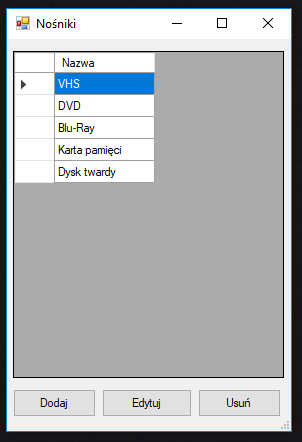
\includegraphics[width=4cm]{carrier.PNG}
\caption{Stworzone okno dla pojedynczych pól. Tutaj Nośniki}
\end{figure}
Mamy opcję dodania pojedynczej właściwości lub jej edycji. W przypadku tworzenia nowego, wyskoczy nam okno, które będzie dziedziczyć po klasie \textit{AddSingleProperty}, która jest oknem bazowym dla wszystkich tabel wymienionych wcześniej. 
\begin{figure}[!ht]
\centering
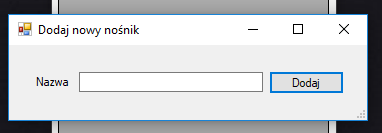
\includegraphics[width=8cm]{addcarrier.PNG}
\caption{Okno dodawania nośnika}
\end{figure}

W przypadku gry będzie chodziło nam o edycję, odpowiednio okno będzie miało zmienioną nazwę (tutaj Edytuj nośnik X) oraz zmieniony napis na przycisku, natomiast w textBoxie ukaże się nam właściwość do wyedytowania. Okno posiada również blokadę, ażeby nie wpisać dwóch tych samych nazw do tabel; dzieje się tak zarówno w przypadku dodawania jak i edycji.
\newpage
\subsection{Filmy (egzemplarze)}
Kolejnym oknem będą filmy, które są aktywne (istnieją aktywne egzemplarze tytułów). W przypadku gdy dany film jest wypożyczony, przycisk "Wypożycz" jest nieaktywny. Ponadto jest możliwość dodania kolejnych egzemplarzy, a w przypadku administratora; jest możliwość edycji i oznaczania filmów jako nieaktywne. Z założenia, filmu nieaktywnego nie da się przywrócić, należy wtedy dodać nowy. 
\begin{figure}[!ht]
\centering
  \begin{subfigure}[b]{0.45\textwidth}
  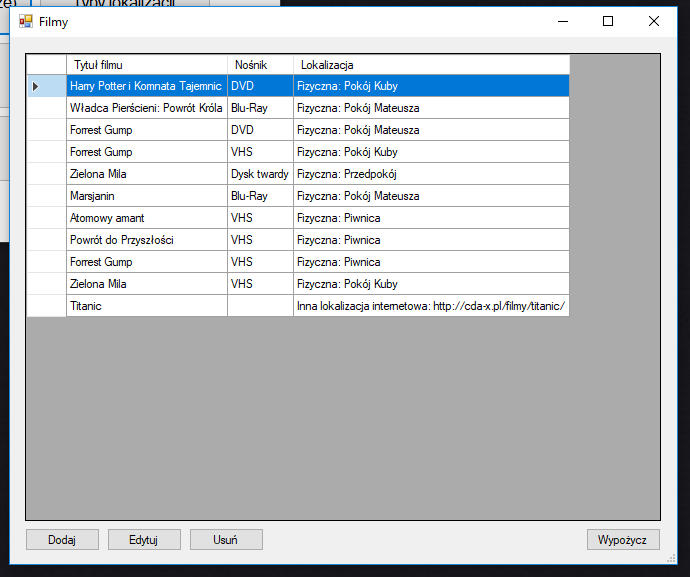
\includegraphics[width=\textwidth]{films.PNG}
  \caption{Filmy}
  \end{subfigure}
  \begin{subfigure}[b]{0.45\textwidth}
  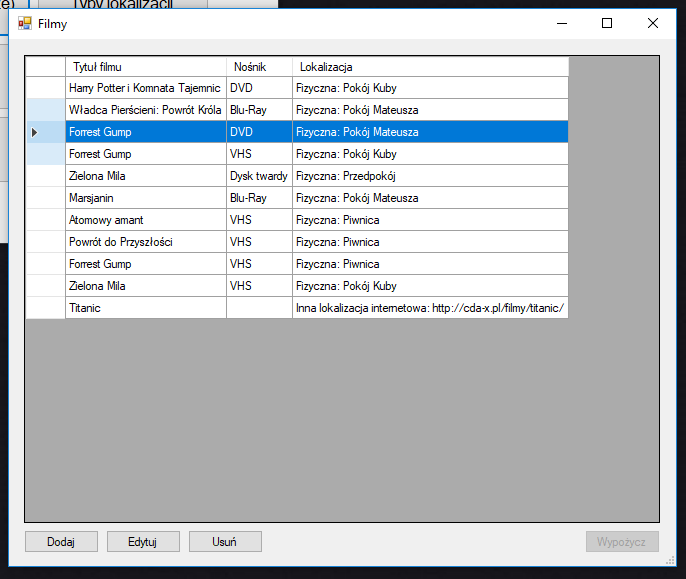
\includegraphics[width=\textwidth]{borrowed.PNG}
  \caption{Wypożyczony film}
  \end{subfigure}
  \caption{Okno Filmy}
\end{figure}
\subsection{Wypożyczenia}
Ostatnim oknem opisywanym w tym dokumencie są wypożyczenia. Po raz kolejny mamy tutaj komponent dataGridView, który zawiera podstawowe dane nt. pożyczonej pozycji. Dla zwykłego użytkownika pojawiają się pozycje, które zostały przez niego wypożyczone - nie widzi on pozycji wypożyczonych przez innych lokatorów. Poniżej grida mamy również przycisk "Zwróć", który odpowiada za usunięcie wskazanego rekordu z tabeli \textit{Hires}. Administrator ma również komponent typu comboBox, z którego może wybrać użytkownika i administracyjnie zwrócić jego wypożyczenia (również swoje). 
\begin{figure}[!ht]
\centering
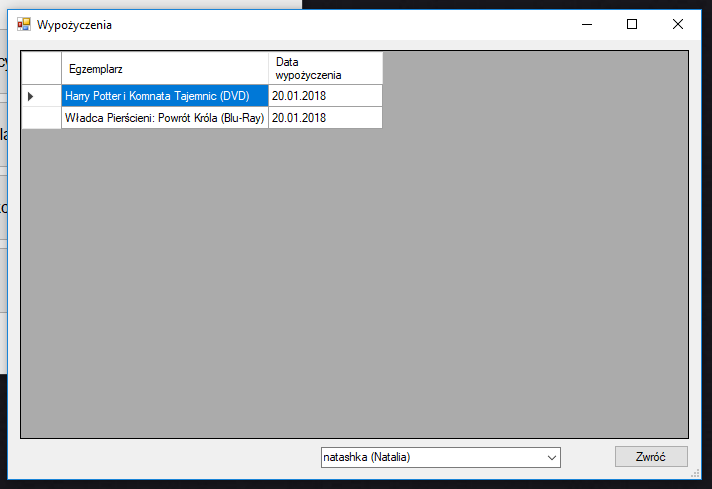
\includegraphics[width=14cm]{hires.PNG}
\caption{Okno wypożyczeń z poziomu panelu administratora}
\end{figure}
\section{Testy aplikacji}
Testy przeprowadziliśmy na bazie oraz w aplikacji. Polegały one na tym, że wpisywaliśmy wybrane dane.
W bazie danych wyjątki były wyrzucane, kiedy były zostawione puste pola w miejscach, gdzie było zaznaczone "not null" oraz kiedy w miejsce integerów były wpisywane wyrazy. 
W aplikacji testy wyglądały podobnie, tylko że wszystkie te wyjątki zostały wyłapane, a użytkownik został poinformowany, że należy zmienić format tekstu lub że nie może zostawić pustego pola.
\section{Podsumowanie}
Nasz projekt był czasochłonny. Należało najpierw przemyśleć, co chcemy zrobić, potem wykonać diagramy, zaprojektować bazę danych, napisać aplikację oraz sprawdzić, czy metody zostały poprawnie zaimplementowane.
	Mogliśmy się nauczyć, jak wygląda tworzenie aplikacji oraz co potrzebujemy do jej wykonania.
	Wartościowe było poznanie możliwości haszowania haseł oraz podejrzenia danych w Wiresharku, jaki to ma skutek.
	Do pozytywnych rzeczy możemy także zaliczyć stawianie bazy danych na maszynie wirtualnej.
	Mamy nadzieję, że trudności na jakie się natchnęliśmy oraz zdobyta wiedza pomogą nam w przyszłości na tworzenie lepszych projektów. 
	
	Nie zamieszczamy żadnej literatury i źródeł, ponieważ z nich nie korzystaliśmy. Nasz projekt powstał na bazie wiedzy nabytej podczas toku studiów oraz w czasie pracy.
\end{document}
